\chapter{Web portal: an aggregator of digital musical heritage collections}\label{ch:portal}
%\todo[inline,author=Enrico]{Shall we move this into a separate section?}
%\todo[inline]{Please provide a summary of the pilot objectives, beneficiaries, and a description of the work done so far, with particular reference to collaborative work and exchange of expertise.}

The Polifonia Web portal is designed to be the main access point to data collections produced in the pilots. 
The objectives of the portal are threefold: (1) to provide user-friendly interfaces and let the general public access valuable information on musical heritage, (2) address exploratory and analytical tasks targeted on specific scholarly groups, and (3) provide access and foster reuse of data sources.

The design and development of the Web portal is iteratively informed by activities carried out by working groups, namely:

\begin{itemize}
    \item Data layer requirements (WP1, WP5, TB)
    \item Software solutions (WP7, TB)
    \item Infrastructure requirements (TB, project coordinator)
    \item Sustainability plans (TB, project coordinator, third-parties)
\end{itemize}
 
\textbf{Data layer requirements.} The socio-technical roadmap (see Deliverable D1.1) offers an overview of \emph{contents} relevant to pilots. It identifies shareable metadata, multi-modality aspects, and linking between data sources to be produced by project members and sources already available on the web. The roadmap provides us with the big picture of content requirements, possible overlaps between data created by pilots, and whether the development and access to certain data sources must be prioritised.

% add also user stories here?

Interviews with scholars participating in music research are carried out to by OU and UNIBO in order to frame the following aspects: (1) data-driven research questions, (2) \emph{data-sense making activities}, and (3) metadata requirements. Domain experts involved in Polifonia pilots are asked to detail their research methods, whether sources are already digitised or not, and whether computer-aided tasks are in scope. Content analysis of transcribed interviews is performed to frame research methods into sense-making primitives and define requirements of the final web interfaces. The latter include tools for exploratory data visualisation (EDA), features of the search engine, and User eXperience (UX) aspects. 

\textbf{Software solutions.} Software solutions that are part of Polifonia ecosystem (see section \ref{ch:ecosystem}) are constantly surveyed by members of the technical board to frame the state of the art, and if needed, propose a intervention of Polifonia developers to fill the gaps. Software solutions include, among the others, (1) \emph{ontologies and vocabularies} that Polifonia data sources rely on (data layer), (2) \emph{software libraries} for Web development, data processing, and Linked Open Data manipulation, and (3) \emph{standards} for music annotation.

A working group including representatives of pilots and the TB is dedicated to the development and maintenance of a \emph{registry} of musical resources on the web. The work extends and optimizes the existing musoW registry (\url{https://musow.kmi.open.ac.uk/}). The objectives of this activity are the following: (1) to develop sustainable solutions for updating and maintaining the online registry with metadata about data sources produced by the project, (2) to allow supervised crowdsourcing of metadata of other data sources and tools relevant to Polifonia objectives and (3) to provide the final web portal with a strategy for harvesting up to date data collections.

Lastly, the activity is informed by the outputs of the Data Management Plan, which details \emph{data publication and dissemination strategies}. Such strategies are iteratively refined according to data volume and long-term preservation purposes, and affect the way the web portal accesses the data layer. 

\textbf{Infrastructure requirements.} The TB defines suitable hosting and deployment solutions to guarantee optimal usage of available resources. We expect infrastructure requirements to vary along with the evolution of data layer requirements. Our work is inspired by previous works addressing similar situations \cite{kirstein2019european,kirstein2020piveau}, namely: distributed systems leveraging data sources stored in different locations, systematically updated by providers, and served according to different access and licensing options.

Fig. \ref{fig:infrastructure} illustrates the high-level infrastructure of the mid-term/final version of the web portal and the dependencies with Work Packages that are involved.

\begin{figure}
    \centering
    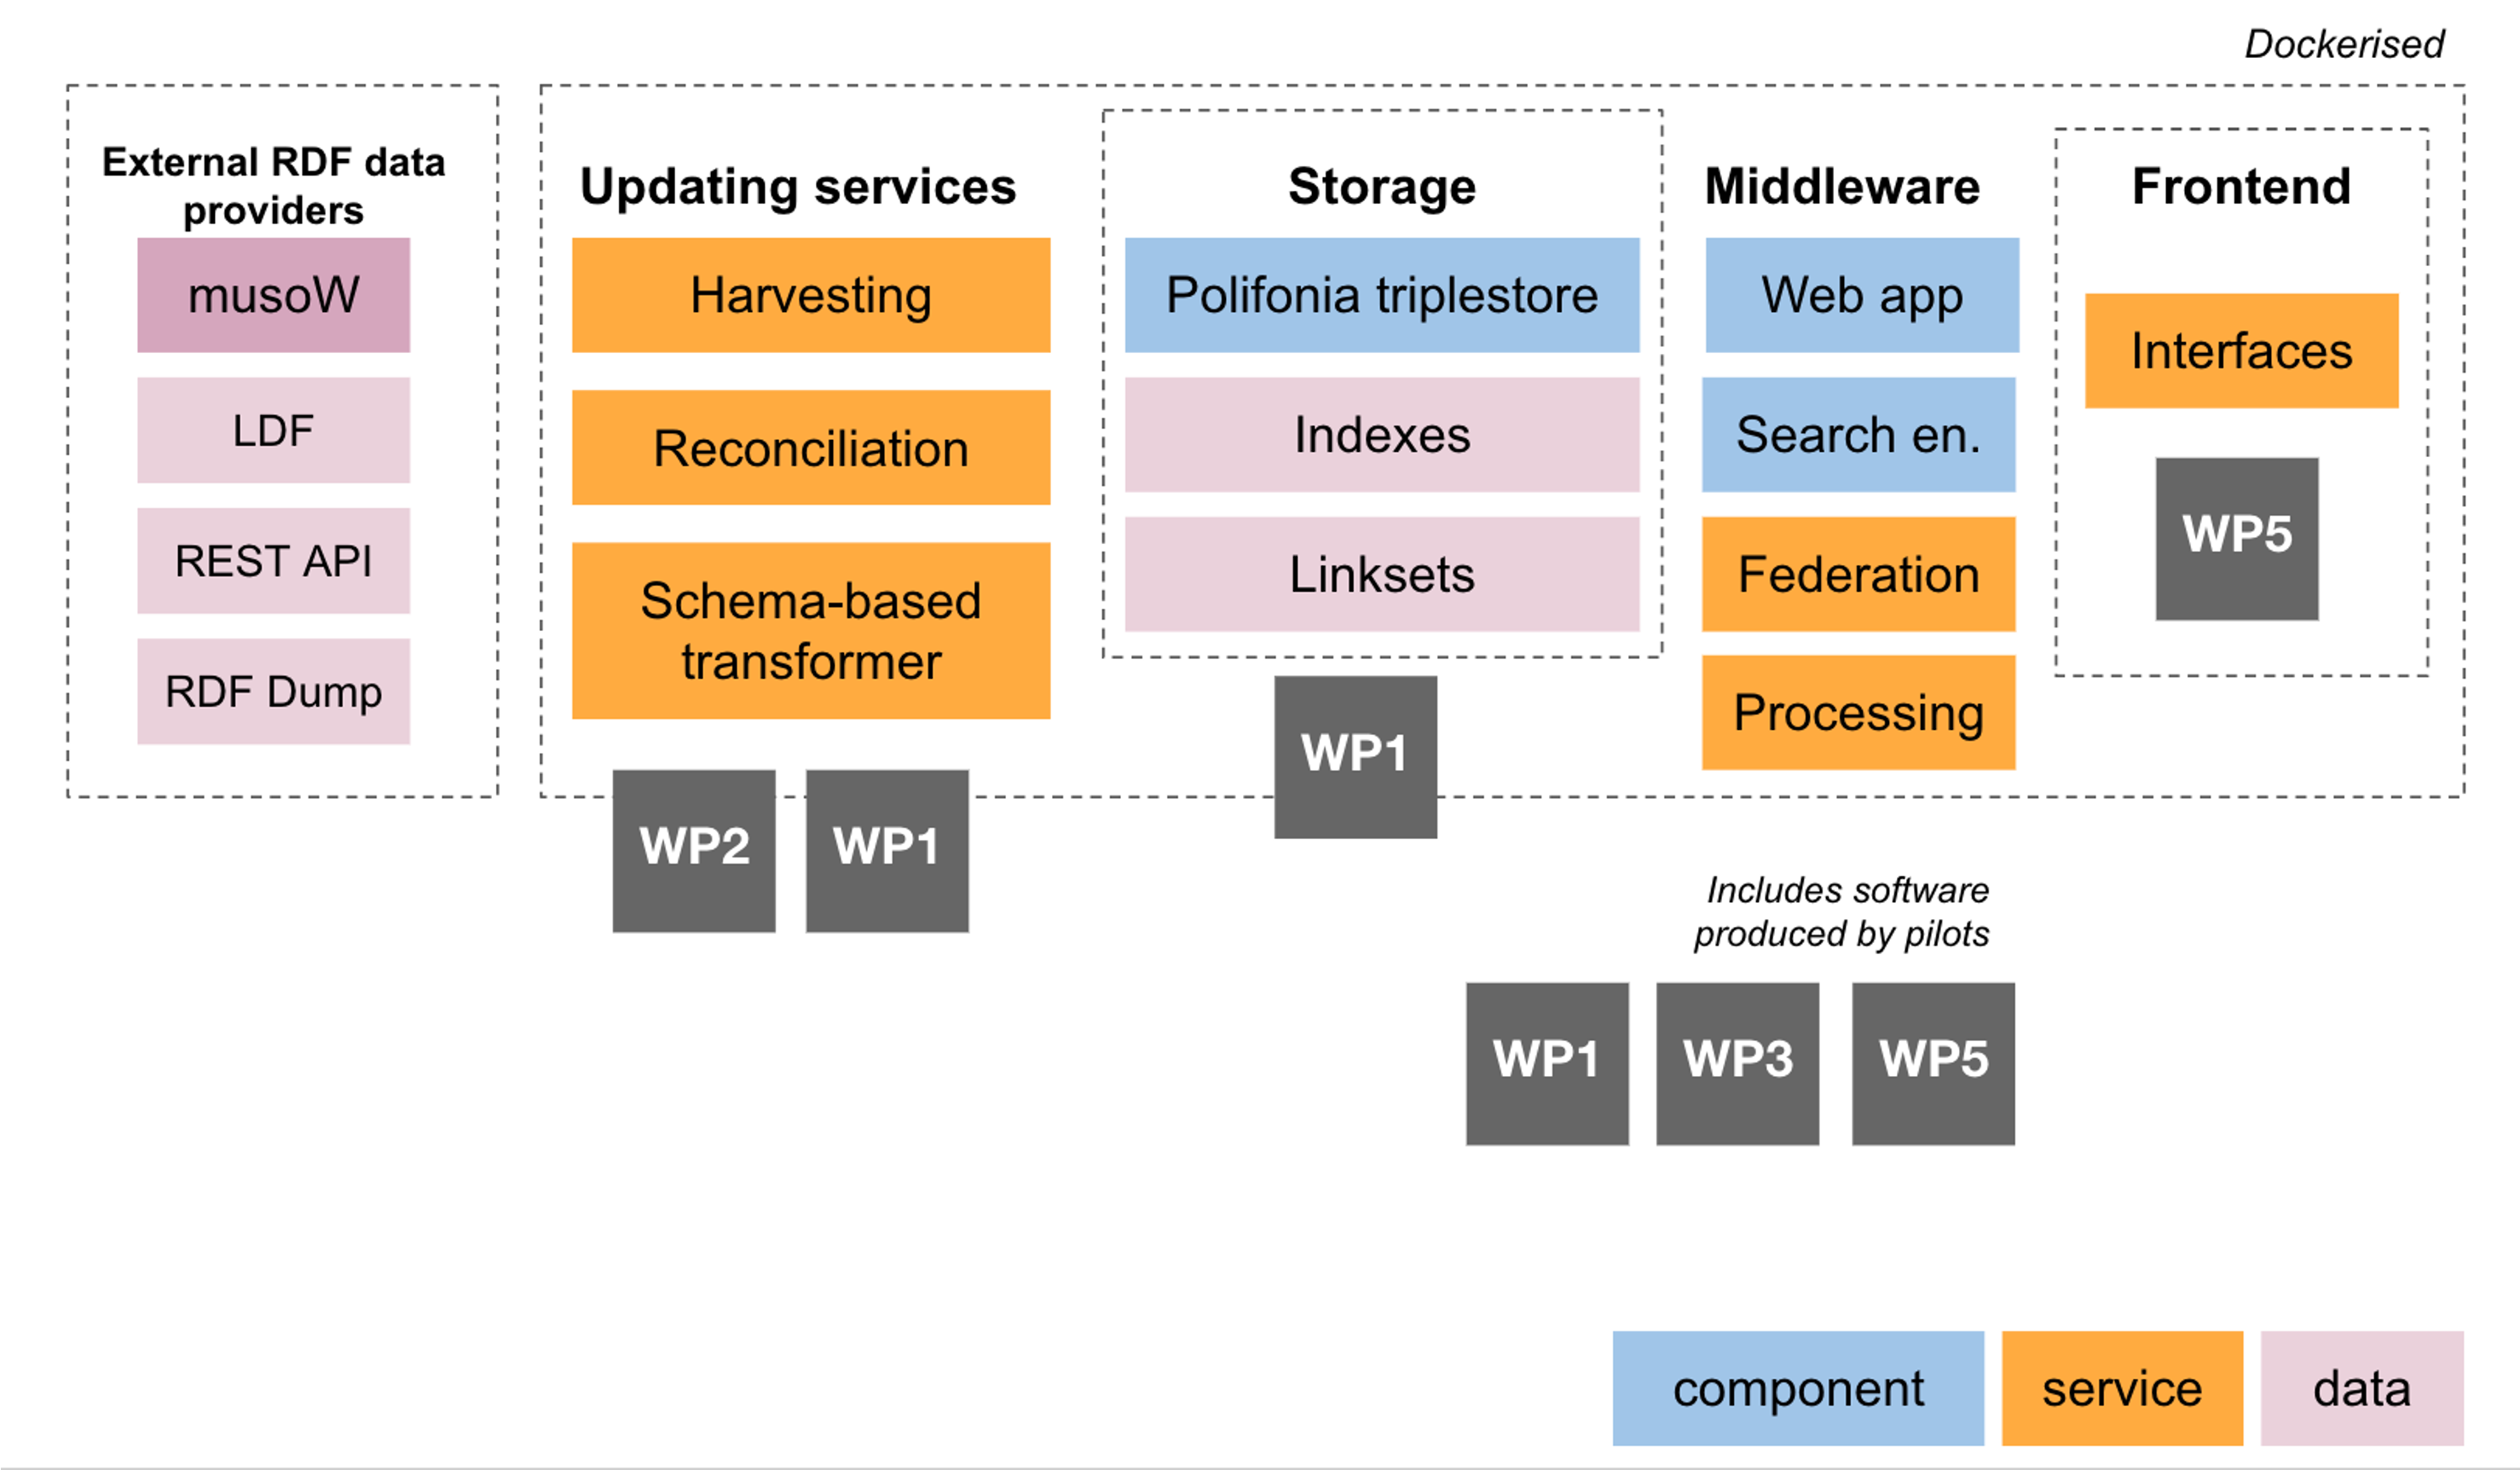
\includegraphics[width=0.7\textwidth]{images/webportal.png}
    \caption{Overview of Polifonia Web Portal infrastructure}
    \label{fig:infrastructure}
\end{figure}

% source of figure (slide 4): https://docs.google.com/presentation/d/1CWxGaiVnrQlq0oqxy4JiNJqwCuIFCuiK99HaoiEv2Ko/edit?usp=sharing

As shown in the picture, we expect data sources to be shared by partners and external data providers in different ways, including SPARQL endpoints, REST APIs, Linked Data Fragments, and RDF data dumps. Among the sources, the musoW catalogue acts as a centralised registry recording cataloguing data of sources that will populate the web portal. 

The web portal back-end includes a dedicated triplestore, which stores selected information harvested from data sources in the form of indexes and linksets. Specialised services perform pre-processing (cleaning), reconciliation (deduplication), and transformation activities (according to a crawling schema). 

The middleware consists of a fully compliant Model-View-Controller (MVC) application, which handles the search engine, federated queries to external sources (when applicable), post-processing of data, and serves data as views.

To deploy and deliver software quickly we use Docker.\footnote{\url{https://www.docker.com}}

\textbf{Sustainability plans} The project coordinator investigates sustainability plans for the Polifonia web portal, with support from the TB. In particular, options for \emph{long-term access, hosting, and maintenance}, of the web portal and data sources may involve third-parties interested in contributing with trusty solutions. 

It is worth noting that one of the advantages of relying on Linked Open Data and Semantic Web technologies includes the usage of \emph{persistent, dereferenceable HTTP URIs} for identifying resources, web documents, and data collections. That is, a end user will always be able to access web resources by using the same persistent URIs regardless their actual location and storage solutions. So doing, we plan to iteratively increment infrastructure requirements without affecting data access and reuse strategies.

\todo[inline,author=Enrico]{Discuss opportunities of presenting views on the Polifonia Website and eventually incorporate actions linked to the portal on that website}